\documentclass[11pt,a4paper]{article}
\usepackage[utf8]{inputenc}
\usepackage[spanish]{babel}
\usepackage{amsmath}
\usepackage{amsfonts}
\usepackage{amssymb}
\usepackage{graphicx}
\usepackage[left=1.2cm,right=1.2cm,top=2cm,bottom=2cm]{geometry}
\date{\small{\today}}
\usepackage{fancyhdr}
\usepackage{afterpage}
\usepackage{titlesec}
\usepackage{float}
\usepackage{gensymb}
\usepackage{xfrac}
\usepackage{tabularx}
\usepackage{multicol}
\usepackage[font=small]{caption}
\usepackage{scrextend}
\usepackage[toc,page]{appendix}
\usepackage{tikz}
\usepackage{tkz-euclide}
\usepackage[siunitx,americanvoltages,fulldiodes]{circuitikz}
\usepackage{stackengine}
\usepackage{mathtools}
\DeclarePairedDelimiter\abs{\lvert}{\rvert}%
\DeclarePairedDelimiter\norm{\lVert}{\rVert}%

\renewcommand\appendixpagename{Apéndices}
\renewcommand\appendixname{Apéndice}

\DeclareMathOperator{\arctantwo}{arctan2}

\titleformat{\section}{\Large\bfseries}{}{0em}{}[]
\titleformat{\subsection}{\large\bfseries}{}{0em}{}[]
\titleformat{\subsubsection}{\bfseries}{}{0em}{}[]
\titleformat{\chapter}{\large\bfseries}{}{0em}{}[]


\setlength\parindent{0pt}


\begin{document}
\title{Adaptación de Impedancia en Guía de Onda Rectangular}
	\LARGE{\textsc{Laboratorio II}}\\
	\Large{Adaptación de Impedancia en Guía de Onda Rectangular}\\
\begin{large}
\small\textsc{Bercic, Jerónimo}\\
\small\textsc{Roqueta, Matías Daniel}\\
\small{Instituto Balseiro, Centro Atómico Bariloche, Comisión Nacional de Energía Atómica}\\
\end{large}
\setcounter{page}{1}

\lhead{Laboratorio II}%Materia
\rhead{Adaptación de Impedancia en Guía de Onda Rectangular}%Título 
\chead{}

\lfoot{J. Bercic, M. Roqueta}
\cfoot{Instituto Balseiro} 
\rfoot{\thepage} 
\renewcommand{\headrulewidth}{0.4pt} 
\renewcommand{\footrulewidth}{0.4pt} 
\pagestyle{fancy}

\hrule
\normalsize
\section{Resumen}

\begin{multicols}{2}
\section{Introducción}
Una guía de ondas electromagnéticas es un dispositivo que se utiliza para restringir la energía de una onda, y que ésta sea propagada en una dirección deseada. De esta manera se puede aprovechar dicha energía de manera más eficiente. Su utilidad es evidente, por ejemplo, en la fabricación de antenas, donde se busca que la propagación sea en una dirección específica y que las pérdidas de información sean mínimas. En la Figura 1 se muestra una guía de ondas electromagnéticas rectangular.
\begin{center}
    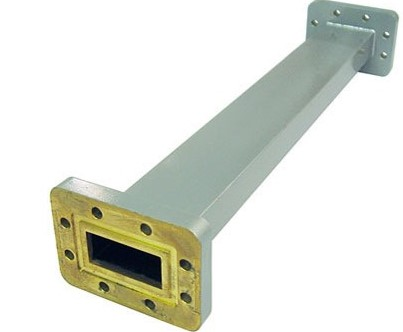
\includegraphics[scale=0.4]{images/Imagen1.jpg} \\
    \textbf{Figura 1}. Guía de ondas electromagnéticas rectangular.
\end{center}
Dentro del contexto de éste tipo de guía de ondas, se encuentran los que se conocen como modos TE$_{mn}$ (Transverse Electric Field) y TM$_{mn}$ (Transverse Magnetic Field), que se refieren a si la onda transversal a la dirección de propagación es la eléctrica o la magnética, respectivamente, $m$ es el número de medias-ondas a lo largo de la guía, y $n$ es el número de medias-ondas a lo alto de la guía. En la Figura 2 se presenta un esquema de una guía de ondas cuyo modo es el TE$_{10}$.
\begin{center}
    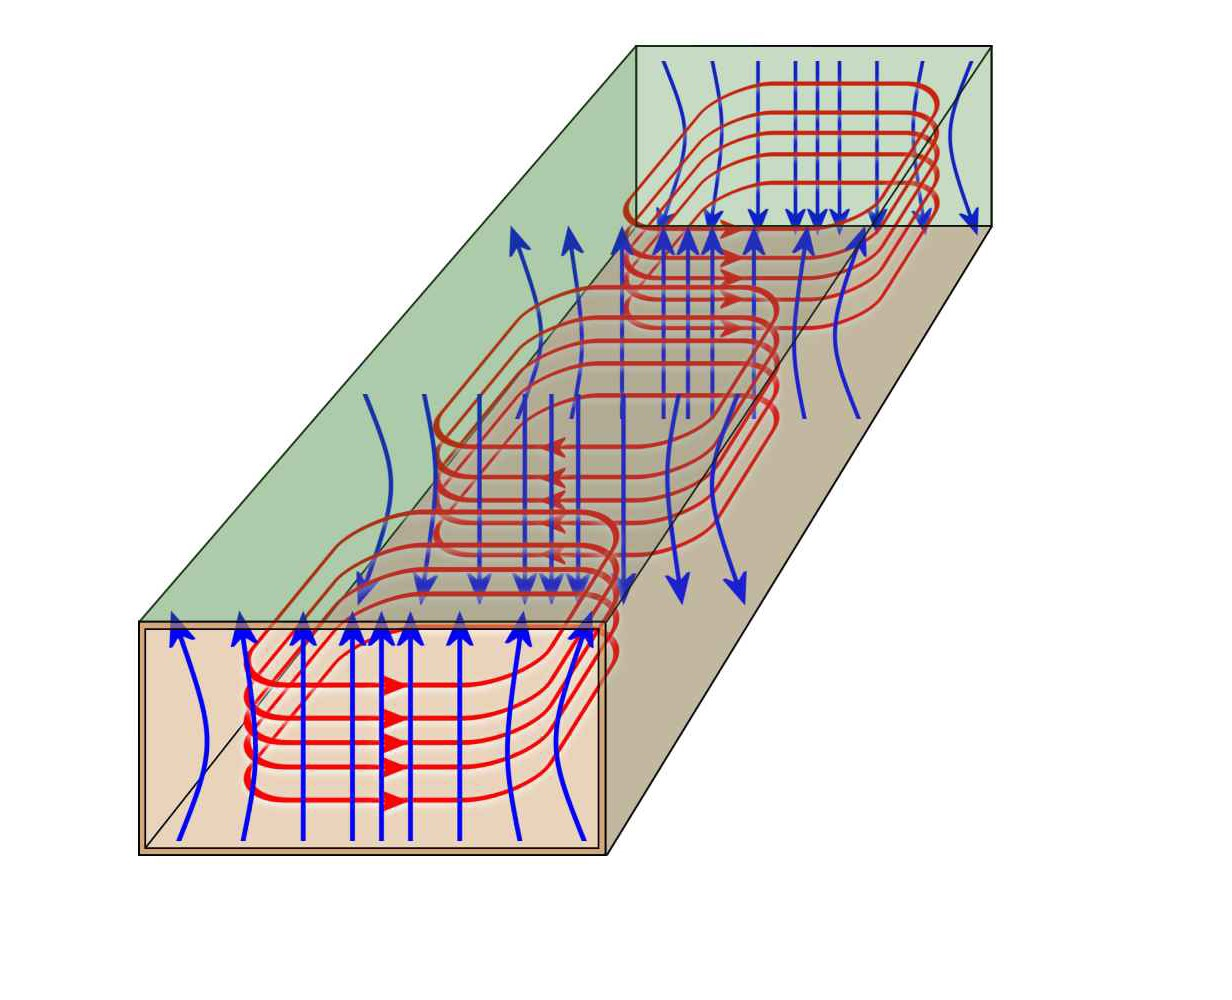
\includegraphics[scale=0.15]{images/TE10.jpg} \\
    \textbf{Figura 2}. Guía de ondas electromagnéticas con modo TE$_{10}$.
\end{center}
El modo de propagación dependerá tanto de las dimensiones de la guía, así como de la frecuencia de la onda propagada. \\ \\
Para poder caracterizar la guía de ondas, se puede pensar en ella como una línea de transmisión, o sea, una cascada de cuadripolos (Figura 3) distribuidos a lo largo de la línea.
\begin{center}
\begin{tikzpicture}[scale=0.75]
\draw (1,3) to [L, l_=$L\:dz$] (-2,3);
\draw (1,3) to [C, l_=$C$] (1,1);
\draw[ultra thin, fill=pink,fill opacity=0.15] (-3,0.25) rectangle (2,3.8);
\draw[->] (-2,1) -- (3,1);
\draw[->] (-2,3) -- (3,3);
\draw (-4,1) -- (-2,1);
\draw (-4,3) -- (-2,3);
\draw (-2,3) -- (-2,1);
\node at (-7,1) { };
\draw[->] (-5.5,3) -- node[above] {$i(z,t)$} (-4.2,3);
\draw[->] (3.2,3) -- node[above] {$i(z+dz,t)$} (4.4,3);
\draw[->] (-4.2, 1.2) -- node[left] {$v(z,t)$} (-4.2,2.7);
\draw[->] (3.2, 1.2) -- node[right] {$v(z+dz,t)$} (3.2,2.7);
\end{tikzpicture}
\textbf{Figura 3}: Esquema del modelo de los cuadripolos a disponer en cascada.
\end{center}
Al igual que una línea de transmisión, las guías de ondas cuentan con una impedancia característica $Z_0$, la cual se puede calcular sabiendo la frecuencia $f$ a la que se propaga la onda, de la siguiente forma
\begin{equation}
    Z_0=\frac{Z_\text{vacío}}{\lambda_\text{vacío}}=Z_\text{vacío}\frac{f}{c}
\end{equation}
Donde $Z_\text{vacío}$ es la impedancia característica del vacío, igual a $376.6$ $\Omega$, $\lambda_\text{vacío}$ es la longitud de la onda propagada si ésta se propagase en el vacío, y $c$ es la velocidad de la luz.\\ \\
Sabiendo la impedancia característica de la guía de ondas, se puede adaptar a la impedancia del plano de carga $Z_\text{L}$, y así poder aprovechar de manera más eficiente la energía transmitida. Éste será el caso si $Z_0$ es igual a $Z_\text{L}$. Para saber si la guía está adaptada se utiliza el \textbf{coeficiente de reflexión} $\Gamma$,
\begin{equation}
    \Gamma = \frac{Z_\text{L}-Z_0}{Z_\text{L}+Z_0}
\end{equation}
el cual vale $\Gamma = -1$ para un corto circuito, $\Gamma = 1$ para un circuito abierto, y $\Gamma = 0$ para la guía adaptada. \\ \\ 
Otra forma de verificar si la guía está adaptada, es analizando la onda estacionaria que se forma debido a la reflexión de la onda en el plano de carga (Figura 4).
\begin{center}
    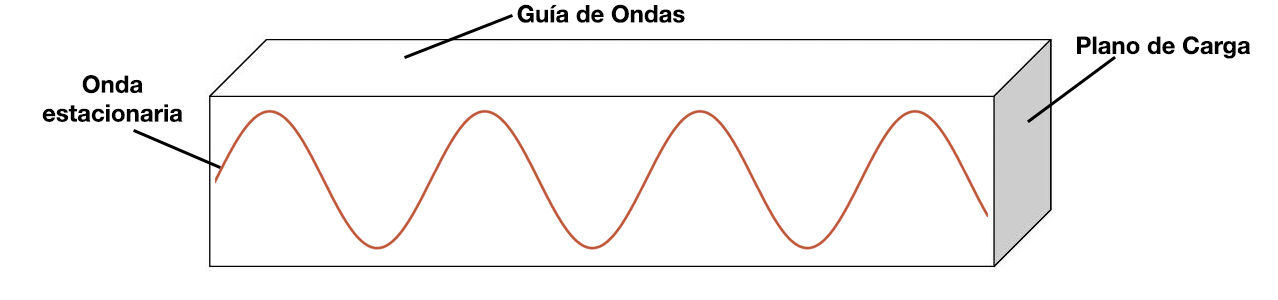
\includegraphics[scale=0.28]{images/Para el informe.jpg} \\
    \textbf{Figura 4}: Onda estacionara formada en la guía debido a la reflexión en el plano de carga. 
\end{center}
Para ello se define el ROE (razón de onda estacionaria) como
\begin{equation}
    \text{ROE} = \frac{1+\abs{\Gamma}}{1-\abs{\Gamma}}
\end{equation}
Este número también se puede calcular haciendo el cociente entre las amplitudes máxima y mínima de la onda estacionaria, y tiene un rango de 
$$
1<\text{ROE} < \infty
$$
Cuanto se quiere adaptar la guía, el ROE debe tender a 1. \\ \\
En este laboratorio, se busca medir las propiedades de la onda estacionaria que se forma bajo distintas condiciones del plano de carga. Además, se busca adaptar la impedancia para ciertas condiciones. 
\section{Método Experimental}

\section{Resultados}


\section{Discusión}

\section{Conclusiones}

\bibliography{LockIn}
\bibliographystyle{unsrt}

\end{multicols}
\newpage
\begin{appendices}
\vspace{-1em}
\hrule
\vspace{1em}
\normalsize
\section{Apéndice 1 -}
\end{appendices}

\begin{multicols}{2}

\end{multicols}

\end{document}